% ----------------------------------------------------------------- %
%             The Speech Signal Processing Toolkit (SPTK)           %
%             developed by SPTK Working Group                       %
%             http://sp-tk.sourceforge.net/                         %
% ----------------------------------------------------------------- %
%                                                                   %
%  Copyright (c) 1984-2007  Tokyo Institute of Technology           %
%                           Interdisciplinary Graduate School of    %
%                           Science and Engineering                 %
%                                                                   %
%                1996-2017  Nagoya Institute of Technology          %
%                           Department of Computer Science          %
%                                                                   %
% All rights reserved.                                              %
%                                                                   %
% Redistribution and use in source and binary forms, with or        %
% without modification, are permitted provided that the following   %
% conditions are met:                                               %
%                                                                   %
% - Redistributions of source code must retain the above copyright  %
%   notice, this list of conditions and the following disclaimer.   %
% - Redistributions in binary form must reproduce the above         %
%   copyright notice, this list of conditions and the following     %
%   disclaimer in the documentation and/or other materials provided %
%   with the distribution.                                          %
% - Neither the name of the SPTK working group nor the names of its %
%   contributors may be used to endorse or promote products derived %
%   from this software without specific prior written permission.   %
%                                                                   %
% THIS SOFTWARE IS PROVIDED BY THE COPYRIGHT HOLDERS AND            %
% CONTRIBUTORS "AS IS" AND ANY EXPRESS OR IMPLIED WARRANTIES,       %
% INCLUDING, BUT NOT LIMITED TO, THE IMPLIED WARRANTIES OF          %
% MERCHANTABILITY AND FITNESS FOR A PARTICULAR PURPOSE ARE          %
% DISCLAIMED. IN NO EVENT SHALL THE COPYRIGHT OWNER OR CONTRIBUTORS %
% BE LIABLE FOR ANY DIRECT, INDIRECT, INCIDENTAL, SPECIAL,          %
% EXEMPLARY, OR CONSEQUENTIAL DAMAGES (INCLUDING, BUT NOT LIMITED   %
% TO, PROCUREMENT OF SUBSTITUTE GOODS OR SERVICES; LOSS OF USE,     %
% DATA, OR PROFITS; OR BUSINESS INTERRUPTION) HOWEVER CAUSED AND ON %
% ANY THEORY OF LIABILITY, WHETHER IN CONTRACT, STRICT LIABILITY,   %
% OR TORT (INCLUDING NEGLIGENCE OR OTHERWISE) ARISING IN ANY WAY    %
% OUT OF THE USE OF THIS SOFTWARE, EVEN IF ADVISED OF THE           %
% POSSIBILITY OF SUCH DAMAGE.                                       %
% ----------------------------------------------------------------- %
\hypertarget{grpdelay}{}
\name{grpdelay}{group delay of digital filter}{signal processing}
\begin{synopsis}
 \item[grpdelay] [ --l $L$ ] [ --m $M$ ] [ --a ] [ {\em infile} ] 
\end{synopsis}

\begin{qsection}{DESCRIPTION}
{\em grpdelay} computes the group delay of a sequence of filter coefficients 
from {\em infile} (or standard input), 
sending the result to standard output.
Input and output data are in float format.
\par
If the {\bf --m} option is omitted
and the length of an input data sequence is less than FFT size,
the input file is padded with 0's and the FFT is evaluated
as exemplified below.
When the {\bf --a} option is given,
the gain is obtained from zero order input.
\par
\[
\begin{array}{lll}
\mbox{Input sequence} & 
\overbrace{\framebox[4.5cm]{$x_0, x_1, \ldots, x_{M}, 0,
					\ldots,0$}}^{L}  & \mbox{filter coefficients}\\
		& \makebox[4.5cm]{0\hfill $L-1$} &
\end{array}
\]
\[
\begin{array}{lll}
\mbox{Output sequence} & \overbrace{\framebox[4.5cm]{$\tau(\omega)$}}^{L/2+1} &
	   \mbox{group delay}\\
		& \makebox[4.5cm]{0\hfill $L-1$} &

\end{array}
\]
\end{qsection}

\begin{options}
	\argm{l}{L}{FFT size power of 2}{256}
	\argm{m}{M}{order of filter}{L-1}
	\argm{a}{}{ARMA filter}{FALSE}
\end{options}


\begin{qsection}{EXAMPLE}
This example plots in the screen the group delay of impulse response
of the filter with the following transfer function.
\begin{displaymath}
  H(z)=\frac{1}{1+0.9z^{-1}}
\end{displaymath}
\begin{quote}
\verb! impulse | dfs -a 1 0.9 | grpdelay | fdrw | xgr !
\end{quote}  
\begin{center}
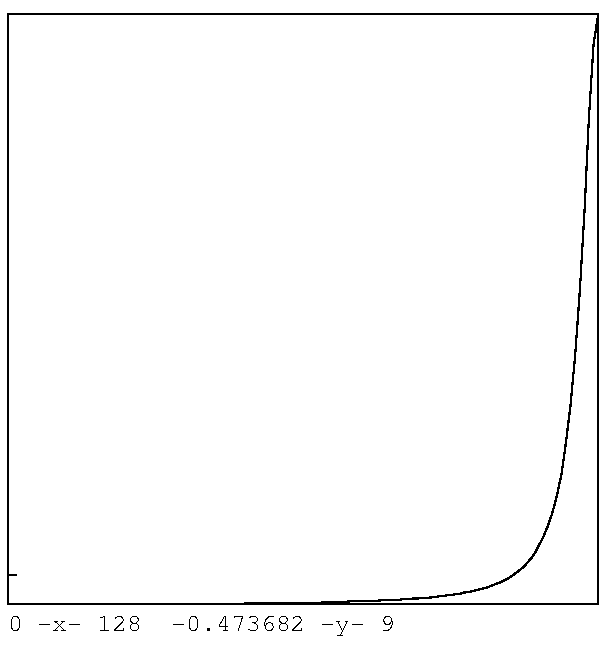
\includegraphics[width=6cm]{fig/grpdelay.pdf}
\end{center}
\end{qsection}

\begin{qsection}{SEE ALSO}
\hyperlink{delay}{delay},
\hyperlink{phase}{phase}
\end{qsection}
